\def\layerA{7}
\def\layerB{9}
\def\layerC{9}
\def\layerD{3}
\def\step{2}
\def\size{3pt}

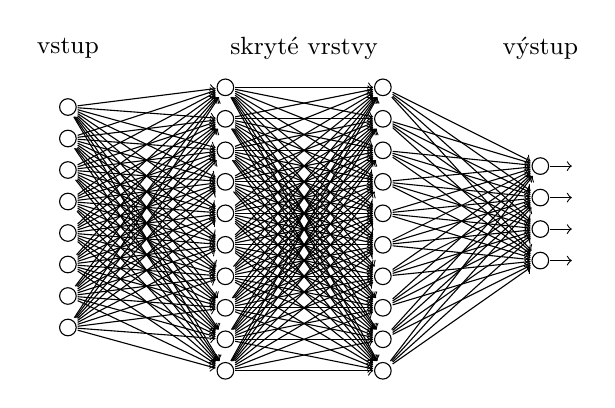
\begin{tikzpicture}[]


\foreach \i in {0,...,\layerA} {
	\draw (0,-0.25 -0.4 * \i) circle (\size) node(layer_1_\i) {};
}
\draw (0, 0.5) node {\small vstup};

\foreach \i in {0,...,\layerB} {
	\draw (\step,-0.4 * \i) circle (\size) node(layer_2_\i) {};
}

\foreach \i in {0,...,\layerC} {
	\draw (2 * \step,-0.4 * \i) circle (\size) node(layer_3_\i) {};
}

\draw (1.5 * \step, 0.5) node {\small skryté vrstvy};

\foreach \i in {0,...,\layerD} {
	\draw (3 * \step,-1 - 0.4 * \i) circle (\size) node(layer_4_\i) {};
    \draw[->] (layer_4_\i) -- (3 * \step + 0.4, -1 - 0.4 * \i);
}

\draw (3 * \step, 0.5) node {\small výstup};

\foreach \i in {0,...,\layerA} {
	\foreach \j in {0,...,\layerB} {
        \draw[->] (layer_1_\i) -- (layer_2_\j);
    }
}

\foreach \i in {0,...,\layerB} {
	\foreach \j in {0,...,\layerC} {
        \draw[->] (layer_2_\i) -- (layer_3_\j);
    }
}

\foreach \i in {0,...,\layerC} {
	\foreach \j in {0,...,\layerD} {
        \draw[->] (layer_3_\i) -- (layer_4_\j);
    }
}

\end{tikzpicture}
